\documentclass[11pt]{article}

\usepackage[a4paper, margin=1in]{geometry}
\usepackage{amsmath, amssymb, graphicx, natbib, hyperref}
\usepackage{authblk}
\usepackage{enumitem}
\usepackage{indentfirst}
\usepackage{booktabs}

% Bold symbols
\newcommand{\bx}{\boldsymbol{x}}
\newcommand{\btheta}{\boldsymbol{\theta}}
\newcommand{\bpi}{\boldsymbol{\pi}}
\newcommand{\bmu}{\boldsymbol{\mu}}
\newcommand{\bsigma}{\boldsymbol{\sigma}}
\newcommand{\bz}{\boldsymbol{z}}
\newcommand{\bphi}{\boldsymbol{\phi}}

% Operators
\newcommand{\pr}{\mathbb{P}}
\newcommand{\ev}{\mathbb{E}}
\newcommand{\var}{\mathbb{V}}

\title{Sampling from Multimodal Posteriors: An Overview}
\author{Ezequiel B. Santos\thanks{ezequiel.braga.santos@gmail.com}}
\affil{School of Applied Mathematics - Getulio Vargas Foundation (FGV EMAp)}
\date{}

\begin{document}

\maketitle

\begin{abstract}

In recent years, Bayesian models have gained significant popularity for their ability to incorporate prior 
knowledge and provide probabilistic interpretations of uncertainty. This is achieved through the use of
Markov Chain Monte Carlo (MCMC) methods, which have been improved and adapted to handle complex posterior
distributions. However, one of the main challenges in Bayesian inference arises from the 
\textit{label switching} problem, particularly in mixture models where the posterior distribution is
multimodal and non-identifiable. This paper provides an overview of the label switching problem, its 
implications for MCMC sampling, and various strategies to address it. We focus on three MCMC methods:
simulated tempering, parallel tempering, and tempered transitions. We illustrate these methods through a
case study using simulated data from a random beta model, comparing the effectiveness of each method in
sampling from the posterior distribution. We also discuss the impact of label switching on posterior inference
and the effectiveness of post-processing techniques to resolve it. Our findings highlight the strengths and
limitations of each method, providing insights into their practical applications in Bayesian inference.

\textbf{Keywords:} Bayesian inference, Markov Chain Monte Carlo, label switching, multimodal posteriors,
mixture models, simulated tempering, parallel tempering, tempered transitions.

\end{abstract}

\section{Introduction}

Bayesian mixture models are widely used for modeling heterogeneous data where observations are assumed to arise 
from multiple latent subpopulations. A common example is the finite mixture of Gaussian distributions, which can 
flexibly approximate complex, multimodal densities. Despite their practical utility, these models pose significant 
computational challenges, particularly in posterior inference via Markov Chain Monte Carlo (MCMC) methods.

One of the main obstacles is the \textit{label switching} problem~\citep{stephens2002dealing}, which arises due to the non-identifiability of 
the mixture components. The likelihood and posterior distributions are invariant to permutations of component 
labels, resulting in a posterior with multiple symmetric modes---one for each of the $K!$ permutations of the 
component labels. Standard MCMC algorithms, such as Gibbs sampling, often struggle to move between these modes, 
leading to poor mixing and biased inference. 

To address this issue, several strategies have been proposed. One class of solutions involves modifying the 
sampling algorithm to better explore multimodal posteriors. Techniques such as \textit{simulated tempering}~
\citep{geyer1995annealing}, \textit{parallel tempering}~\citep{earl2005parallel}, and 
\textit{tempered transitions}~\citep{neal1996sampling} have been developed to improve the mixing of MCMC 
chains in the presence of multiple modes. These methods introduce auxiliary distributions at different 
``temperatures'' to allow the sampler to traverse the posterior landscape more effectively.

Another class of solutions aims to resolve the label switching problem through post-processing, either by imposing 
identifiability constraints or by applying relabeling algorithms that align the sampled parameters across 
iterations~\citep{jasra2005labelswitching}.

In this work, we investigate the performance of different tempering-based MCMC methods for sampling from the 
posterior of a Gaussian mixture model. We simulate data from a known mixture distribution and compare the 
effectiveness of standard Gibbs sampling, parallel tempering, and tempered transitions. We also explore 
post-processing approaches for resolving label switching and assess their impact on the posterior summaries. Our 
goal is to provide a comprehensive comparison of these methods in terms of their ability to explore multimodal 
posteriors, their computational efficiency, and the quality of their inference.


\section{Label Switching}

As defined by Jasra et al.~\citep{jasra2005labelswitching}, let $\bx = (x_1, x_2, \ldots, x_n)$ be 
a random sample from a mixture model with $K$ components:
\begin{align*}
    p(\bx \mid \btheta) &= \prod_{i=1}^n \sum_{k=1}^{K} \pi_k f(x_i \mid \phi_k),
\end{align*}
where $\pi_k$ are the mixing proportions, and $f(x_i \mid \phi_k)$ are the component densities with 
parameters $\phi_k$. We assume $\sum_{k=1}^{K} \pi_k = 1$ and $0 \leq \pi_k \leq 1$ for all $k$.

Let $\btheta = \left( (\pi_1, \phi_1), \ldots, (\pi_K, \phi_K) \right)$, and let $\sigma \in S_K$ 
be a permutation of $\{1, \ldots, K\}$. Then,
\begin{align*}
    \sigma(\btheta) &= \left( \theta_{\sigma(1)}, \ldots, \theta_{\sigma(K)} \right).
\end{align*}

The \emph{label switching} problem arises because the likelihood and posterior are invariant to 
such permutations. That is,
\begin{align*}
    p(\bx \mid \sigma(\btheta)) &= \prod_{i=1}^{n} \sum_{k=1}^{K} \pi_{\sigma(k)} 
    f(x_i \mid \phi_{\sigma(k)}),
\end{align*}
is equal to $p(\bx \mid \btheta)$ for all $\sigma \in S_K$. This symmetry introduces $K!$ identical
modes in the posterior distribution.

\subsection{Example: Random Beta Model}

A classic example is the random beta model, where we consider a mixture of $K$ Normal components
\begin{align*}
    x_i \mid \bpi, \bmu, \bsigma &\sim \sum_{k=1}^{K} \pi_k \operatorname{Normal}(x_i \mid \mu_k, \sigma_k^2),
\end{align*}
with prior distributions
\begin{align*}
    \bpi &\sim \operatorname{Dirichlet}(\alpha_1, \ldots, \alpha_K), \\
    \mu_k &\sim \operatorname{Normal}(m, \tau^2), \\
    \sigma_k^2 &\sim \operatorname{InverseGamma}(a, b),
\end{align*}
for $k = 1, \ldots, K$. These distributions lead to a semi-conjugate prior structure and a posterior
that is multimodal due to label switching.

\section{MCMC for Multimodal Posteriors}

The multimodality caused by label switching creates difficulties for Markov Chain Monte Carlo (MCMC) 
methods. Standard algorithms may get trapped in local modes, resulting in poor mixing and high 
autocorrelation. The most common approach is to use Gibbs sampling, which consists to introduce latent 
variables $\bz = (z_1, \ldots, z_n)$ indicating the component assignments:
\[
    \pr(z_i = k \mid \bpi) = \pi_k.
\]
Then we can compute the full conditional posterior distributions of $(\bz, \bpi, \bphi)$ and iterate
over them. However, the sampler may get stuck in one mode and fail to explore others, making it ineffective 
for label-switching scenarios. Below, we explore how various MCMC techniques handle these challenges and 
illustrate their effectiveness in sampling from a simulated data.

\subsection{Simulated Tempering}

Following the idea proposed by Geyer~\citep{geyer1995annealing}, suppose we want to sample from a 
distribution $P$ with density $p_0(x)$ which is multimodal. We can introduce a sequence of inverse 
temperatures $\beta_i$ to create a family of tempered distributions:
\[
    p_i(x) = \frac{p_0(x)^{\beta_i}}{Z_i},
\]
where $\beta_0 = 1 > \beta_1 > \cdots > \beta_m = \beta^*$ and $Z_i = Z_i(\beta_i) = 
\int p_0(x)^{\beta_i} dx$ is the normalization constant.

The algorithm alternates between:
\begin{enumerate}
    \item Sampling $\btheta$ from $p_i(x)$ using MCMC,
    \item Proposing a change to temperature $j = i \pm 1$ using transition probabilities $q_{ij}$,
    \item Accepting the move with probability:
    \[
        \alpha_{ij} = \min\left(1, \frac{p_j(\btheta)\pi_0(j) q_{ji} }{p_i(\btheta)\pi_0(i) q_{ij} }\right),
    \]
\end{enumerate}
where $\pi_0(i)$ is a pseudoprior over the temperatures. When $q_{ij}$ is
uniform, i.e., $q_{ij} = 1/2$ for $1 < i < m$ and $q_{ij} = 1$ for $i = 1, m$, we can simplify the
acceptance probability.

This method updates the chain in two steps: first, it samples from the tempered distribution
$p_i(x)$, and then it proposes to change the temperature. Then, the invariant distribution of the
chain for a fixed temperature $i$ keeps $p_i(x)$. So a sample from $p_0(x)$ can be obtained by
running the chain for a long time and discarding the samples from $i \neq 0$.

As also noted by Neal~\citep{neal1996sampling}, a common choice is $\pi_0(i) = 1/Z_i$ to assign 
uniform prior probabilities to the temperatures. However, in practice, $Z_i$ is often unknown, and
need to be estimated. This leads to the need for calibration techniques to ensure that the 
temperatures are chosen appropriately to balance exploration and convergence. So the algorithm might
require a large computational cost.

\section{Parallel Tempering}

Alternatively, we can run multiple chains in parallel at different temperatures, known as
\emph{parallel tempering}~\citep{earl2005parallel}. This method consider the same family of tempered
as above, but instead of simulating a single chain, we run $m$ chains at temperatures 
$\beta_1, \ldots, \beta_m$. Each chain samples from the tempered distribution $p_i(x)$. But, instead of
accepting moves between temperatures, we periodically propose to swap states of two chains $(i, j)$: we
sample a pair of chains and propose to swap their states with acceptance probability:
\[
    \alpha_{ij} = \min\left(1, \frac{p_j(x_i) p_i(x_j)}{p_i(x_i) p_j(x_j)}\right).
\]

This procedure does not change the invariant distribution of the chain, as it still samples from
the tempered distributions $p_i(x)$. In particular, the chain at temperature $i= 0$ will converge to
the target distribution $p_0(x)$.

\section{Tempered Transitions}

Another approach to deal with multimodal posteriors is to use \emph{tempered transitions}~
\citep{neal1996sampling}. The idea is to construct kernels $\hat{T}_i$ and $\check{T}_i$ that
simulate forward and backward transitions, respectively, between the states of a Markov chain at
temperatures $i$ and $m-i+1$. The forward kernel $\hat{T}_i$ samples from the tempered distribution
$p_i(x)$, while the backward kernel $\check{T}_i$ samples from $p_{m-i+1}(x)$. They must satisfy the
detailed balance condition:
\[
    \hat{T}_i(x, y) p_i(x) = \check{T}_i(y, x) p_{m-i+1}(y),
\]
where $x, y$ are states of the Markov chain. The algorithm proceeds as follows:

\begin{enumerate}
    \item From $x_t$, simulate $\hat{x}_1, \ldots, \hat{x}_m$ via forward kernels 
    $\hat{T}_i$;
    \item Then simulate $\check{x}_m, \ldots, \check{x}_1, \hat{x}_0$ using 
    backward kernels $\check{T}_i$;
    \item Accept the proposal $\hat{x}_0$ with probability:
    \[
        \alpha = \min\left(1, \frac{\prod_{i=1}^{m} p_i(\hat{x}_{i-1}) \prod_{i=1}^{m} 
        p_{m-i+1}(\check{x}_i)}{\prod_{i=1}^{m} p_i(\check{x}_{i-1}) \prod_{i=1}^{m} 
        p_{m-i+1}(\hat{x}_i)} \right).
    \]
\end{enumerate}

This leads to a Markov chain with invariant distribution $p_0(x)$, as shown by Neal~\citep{neal1996sampling}.

\section{Dealing with Label Switching}

While tempering methods improve exploration, they do not resolve label switching. The posterior 
remains multimodal and non-identifiable. Solutions involve either imposing identifiability 
constraints or using post-processing.

\subsection{Imposing Constraints}

A straightforward solution is to enforce parameter ordering, e.g., 
$\mu_1 < \mu_2 < \cdots < \mu_K$, as in Stephens et al.~\citep{stephens1997bayesian}. After 
sampling, parameters are reordered to match this constraint. However, as discussed by Sperring et al.~
\citep{sperrin2010probabilistic}, although this approach works well in many cases and leads to correct
marginal posterior distributions, it can lead to biased estimates.

\subsection{Relabeling Algorithms}

A more general approach uses relabeling algorithms that minimize an expected loss. Let 
$L_0(a, \sigma(\btheta))$ be a base loss function comparing action $a$ with permuted parameter 
$\sigma(\btheta)$. Define the symmetrized loss:
\[
    L(a, \btheta) = \min_{\sigma \in S_K} L_0(a, \sigma(\btheta)).
\]

Then, the optimal action $a^*$ solves:
\[
    a^* = \arg\min_{a \in \mathcal{A}} \mathbb{E}_{\btheta \sim p(\btheta \mid \bx)}[L(a, \btheta)].
\]

As this expectation is intractable, it is approximated using Monte Carlo methods over MCMC samples. As 
described by Stephens et al.~\citep{stephens2002dealing}, the algorithm proceeds by starting with an
initial guess for the labels, then iteratively minimizes the posterior expected loss until convergence.

\section{Case Study: Simulated Data}

We will simulate data from a random beta model with $K = 4$ components, using the following parameters:
\begin{align*}
    \pi_k &= 0.25, \quad k = 1, \ldots, 4, \\
    \bmu &= (-3, 0, 3, 6), \\
    \sigma_k^2 &= 0.55^2, \quad k = 1, \ldots, 4.
\end{align*}

We will compare the performance of standard Gibbs sampling with tempered transitions and parallel
tempering. The goal is to analyze how well each method explores the multimodal posterior and handles
label switching. We will also visualize the results using trace plots and posterior distributions.

We run all methods for $2 \cdot 10^5$ iterations, discarding the first $5 \cdot 10^4$ as burn-in. Also,
we apply tempered distributions for each conditional posterior, i.e., 
\begin{align*}
    p(\bmu \mid \bx, \bpi, \bsigma^2) &\propto p(\bx \mid \bmu, \bpi, \bsigma^2) p(\bmu), \\
    p(\bsigma^2 \mid \bx, \bmu, \bpi) &\propto p(\bx \mid \bmu, \bpi, \bsigma^2) p(\bsigma^2), \\
    p(\bpi \mid \bx, \bmu, \bsigma^2) &\propto p(\bx \mid \bmu, \bpi, \bsigma^2) p(\bpi),
\end{align*}

because the use of the joint posterior may lead to small acceptance rates, as noted by Jasra et 
al.~\citep{jasra2005labelswitching}. Another important point is that we reparameterize the weights
$\bpi$ using $\pi_k = \nu_k / \sum_{j=1}^{K} \nu_j$, where $\nu_k \sim \operatorname{Gamma}(1, 1)$, 
to avoid issues with proposed values outside the simplex. 

For the proposal distributions, we use a Gaussian random walk for $\bmu$ and reflective random walk for
$\bsigma$ and $\bpi$. The temperature ladder is chosen as $\beta_i = 2^{-i}$ for $i = 0, 1, \ldots, 19$, 
for tempered transitions, and $\beta_0 = 1, \beta_1 = 0.9, \ldots, \beta_{9} = 0.1$ for parallel tempering.
Futhermore, we propose a swap move or run the tempered transitions with probability $0.5$ every iteration. 
For full details on the implementation, see the code repository 
\url{https://github.com/EzequielEBS/multimodal-bayesian-sampling}.

In the figure \ref{fig:data_distribution}, we show the simulated data distribution, which is a mixture of 
four Normal components. The modes are clearly separated, and the data is generated from a well-defined
multimodal distribution.

\begin{figure}[!ht]
    \centering
    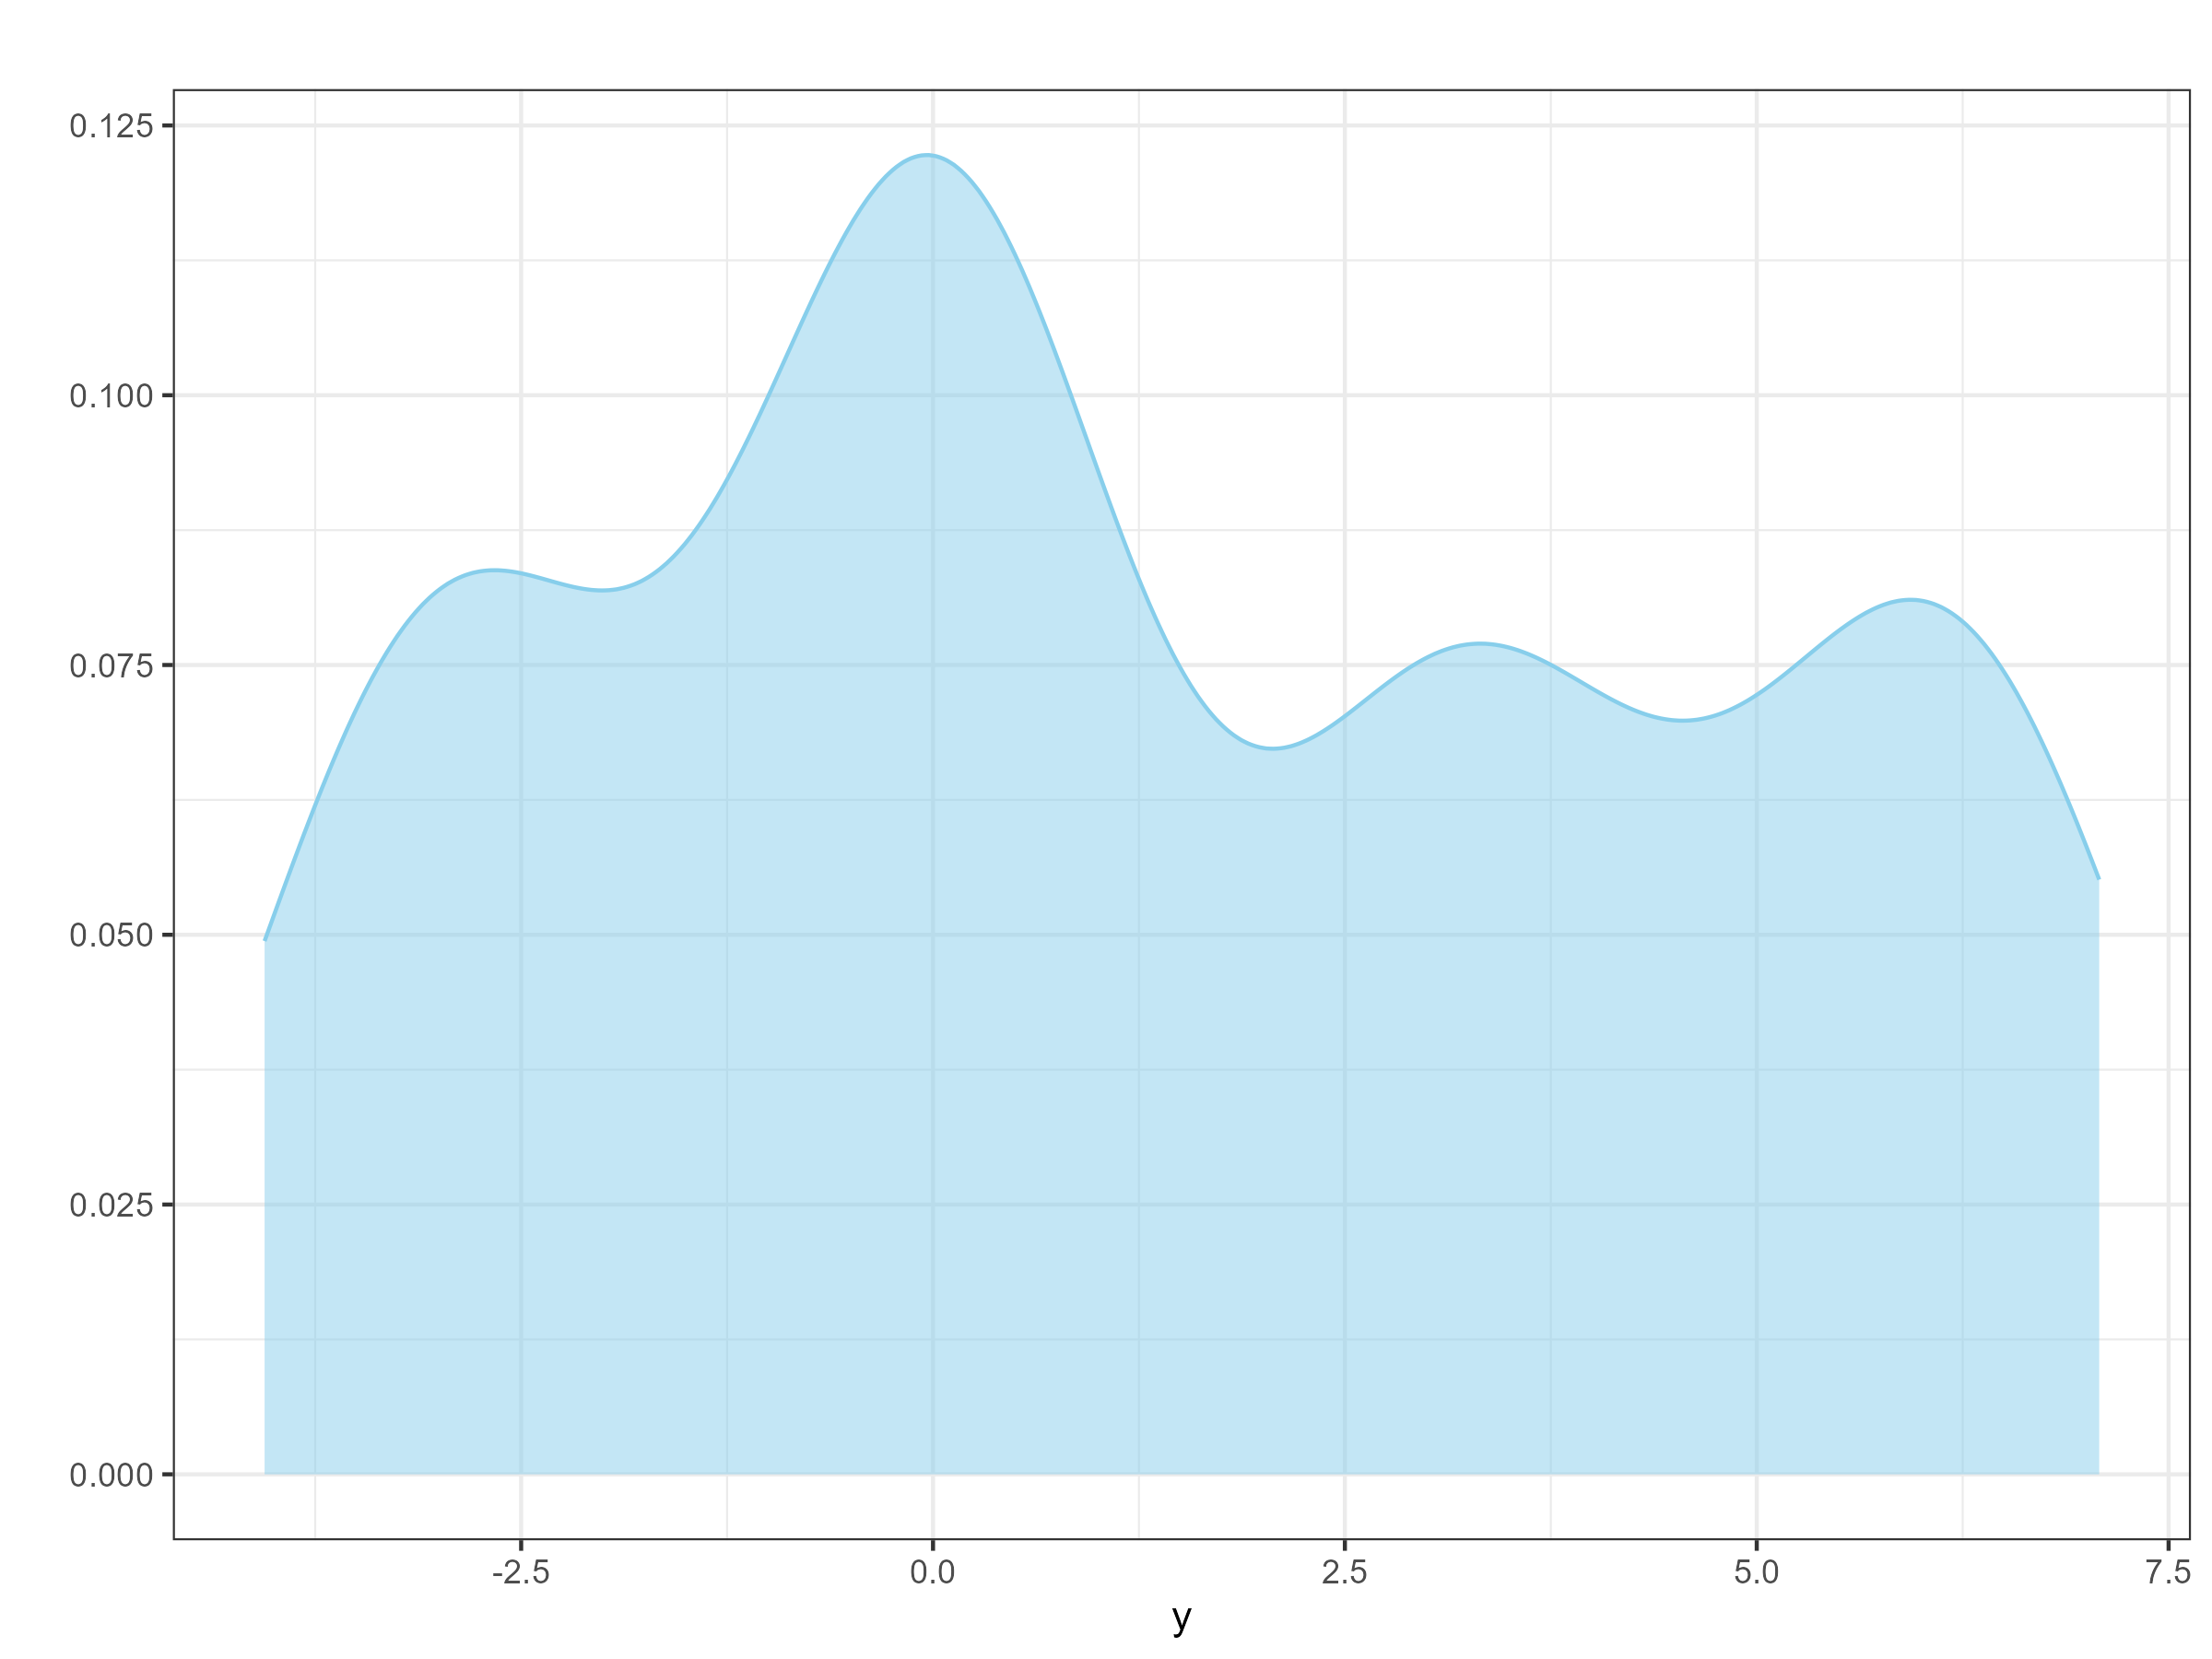
\includegraphics[scale=0.6]{figures/data_plot_random_beta.png}
    \caption{\textbf{Simulated Data Distribution.}}
    \label{fig:data_distribution}
\end{figure}

Also, we show the trace plots for the parameters $\bmu$, $\bsigma^2$, and $\bpi$ obtained from the three methods
in the figures \ref{fig:trace_plots_mu}, \ref{fig:trace_plots_sigma}, and \ref{fig:trace_plots_pi}.

\begin{figure}[!ht]
    \centering
    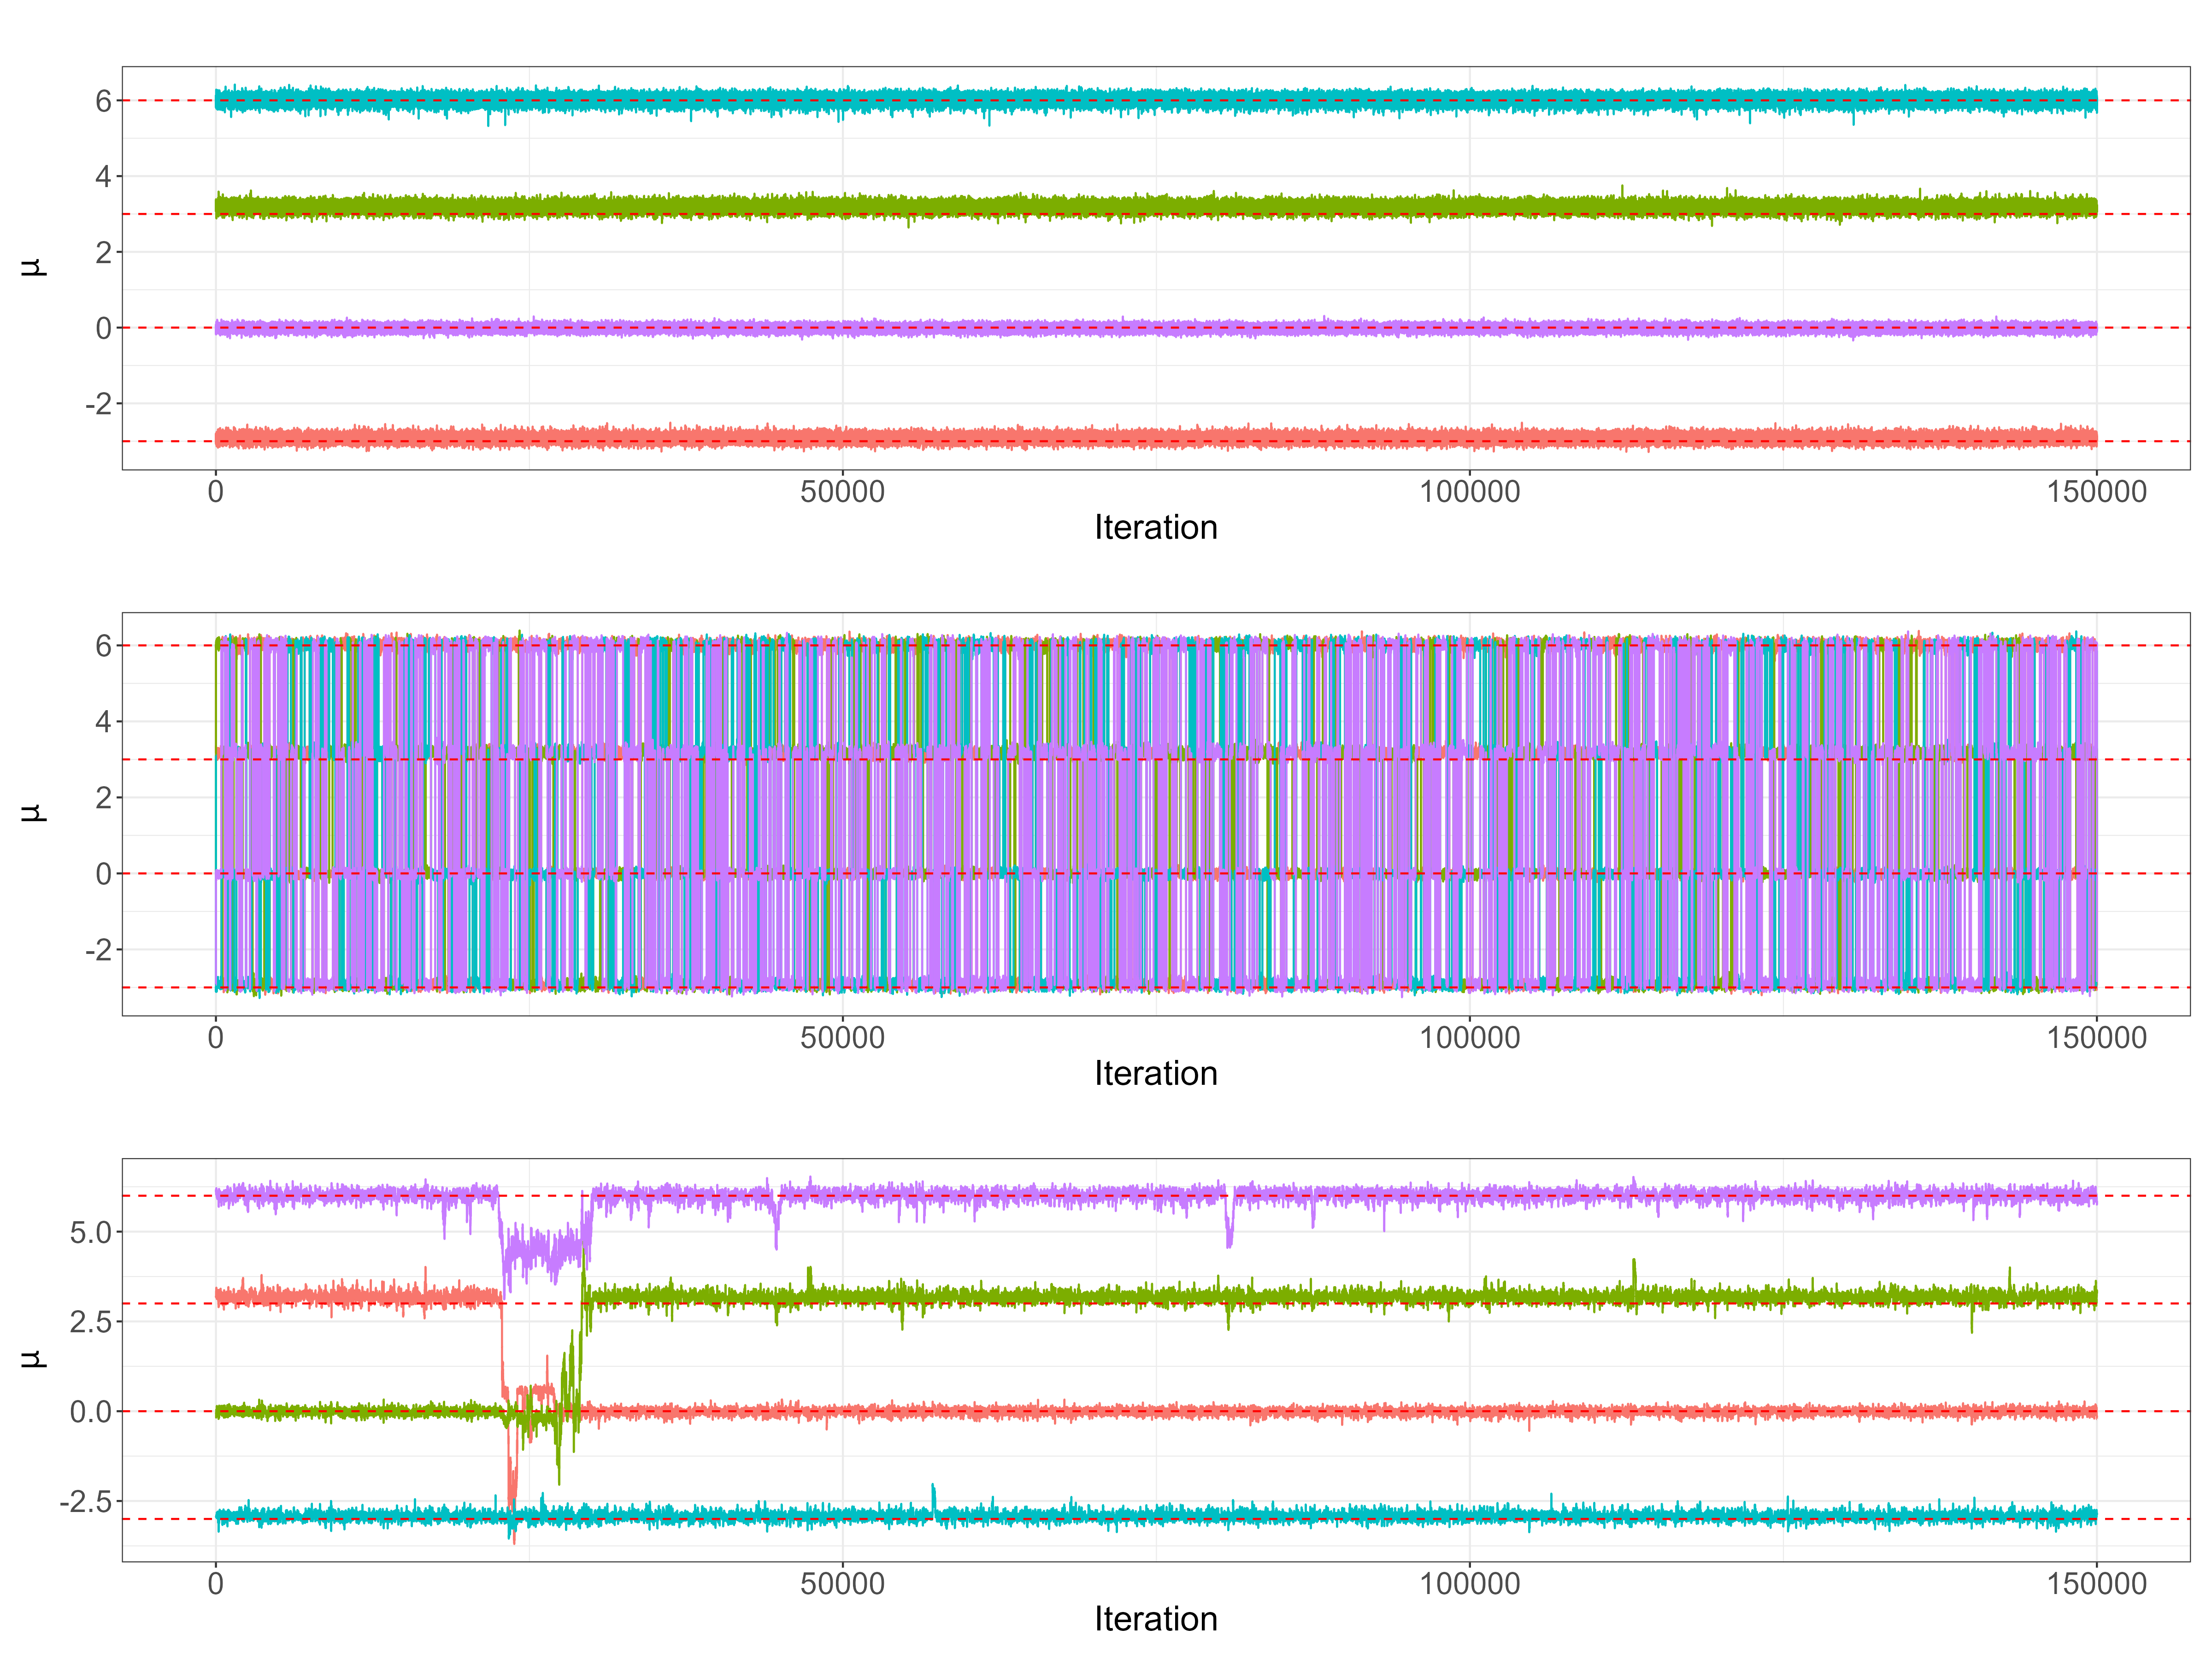
\includegraphics[scale=0.4]{figures/trace_mu_random_beta.png}
    \caption{\textbf{Trace plots for $\bmu$.} The first row shows the trace for Gibbs sampling, the second row for
    parallel tempering, and the third row for tempered transitions. Each color represents a different component. 
    The dashed lines indicate the true parameter values.}
    \label{fig:trace_plots_mu}
\end{figure}

\begin{figure}[!ht]
    \centering
    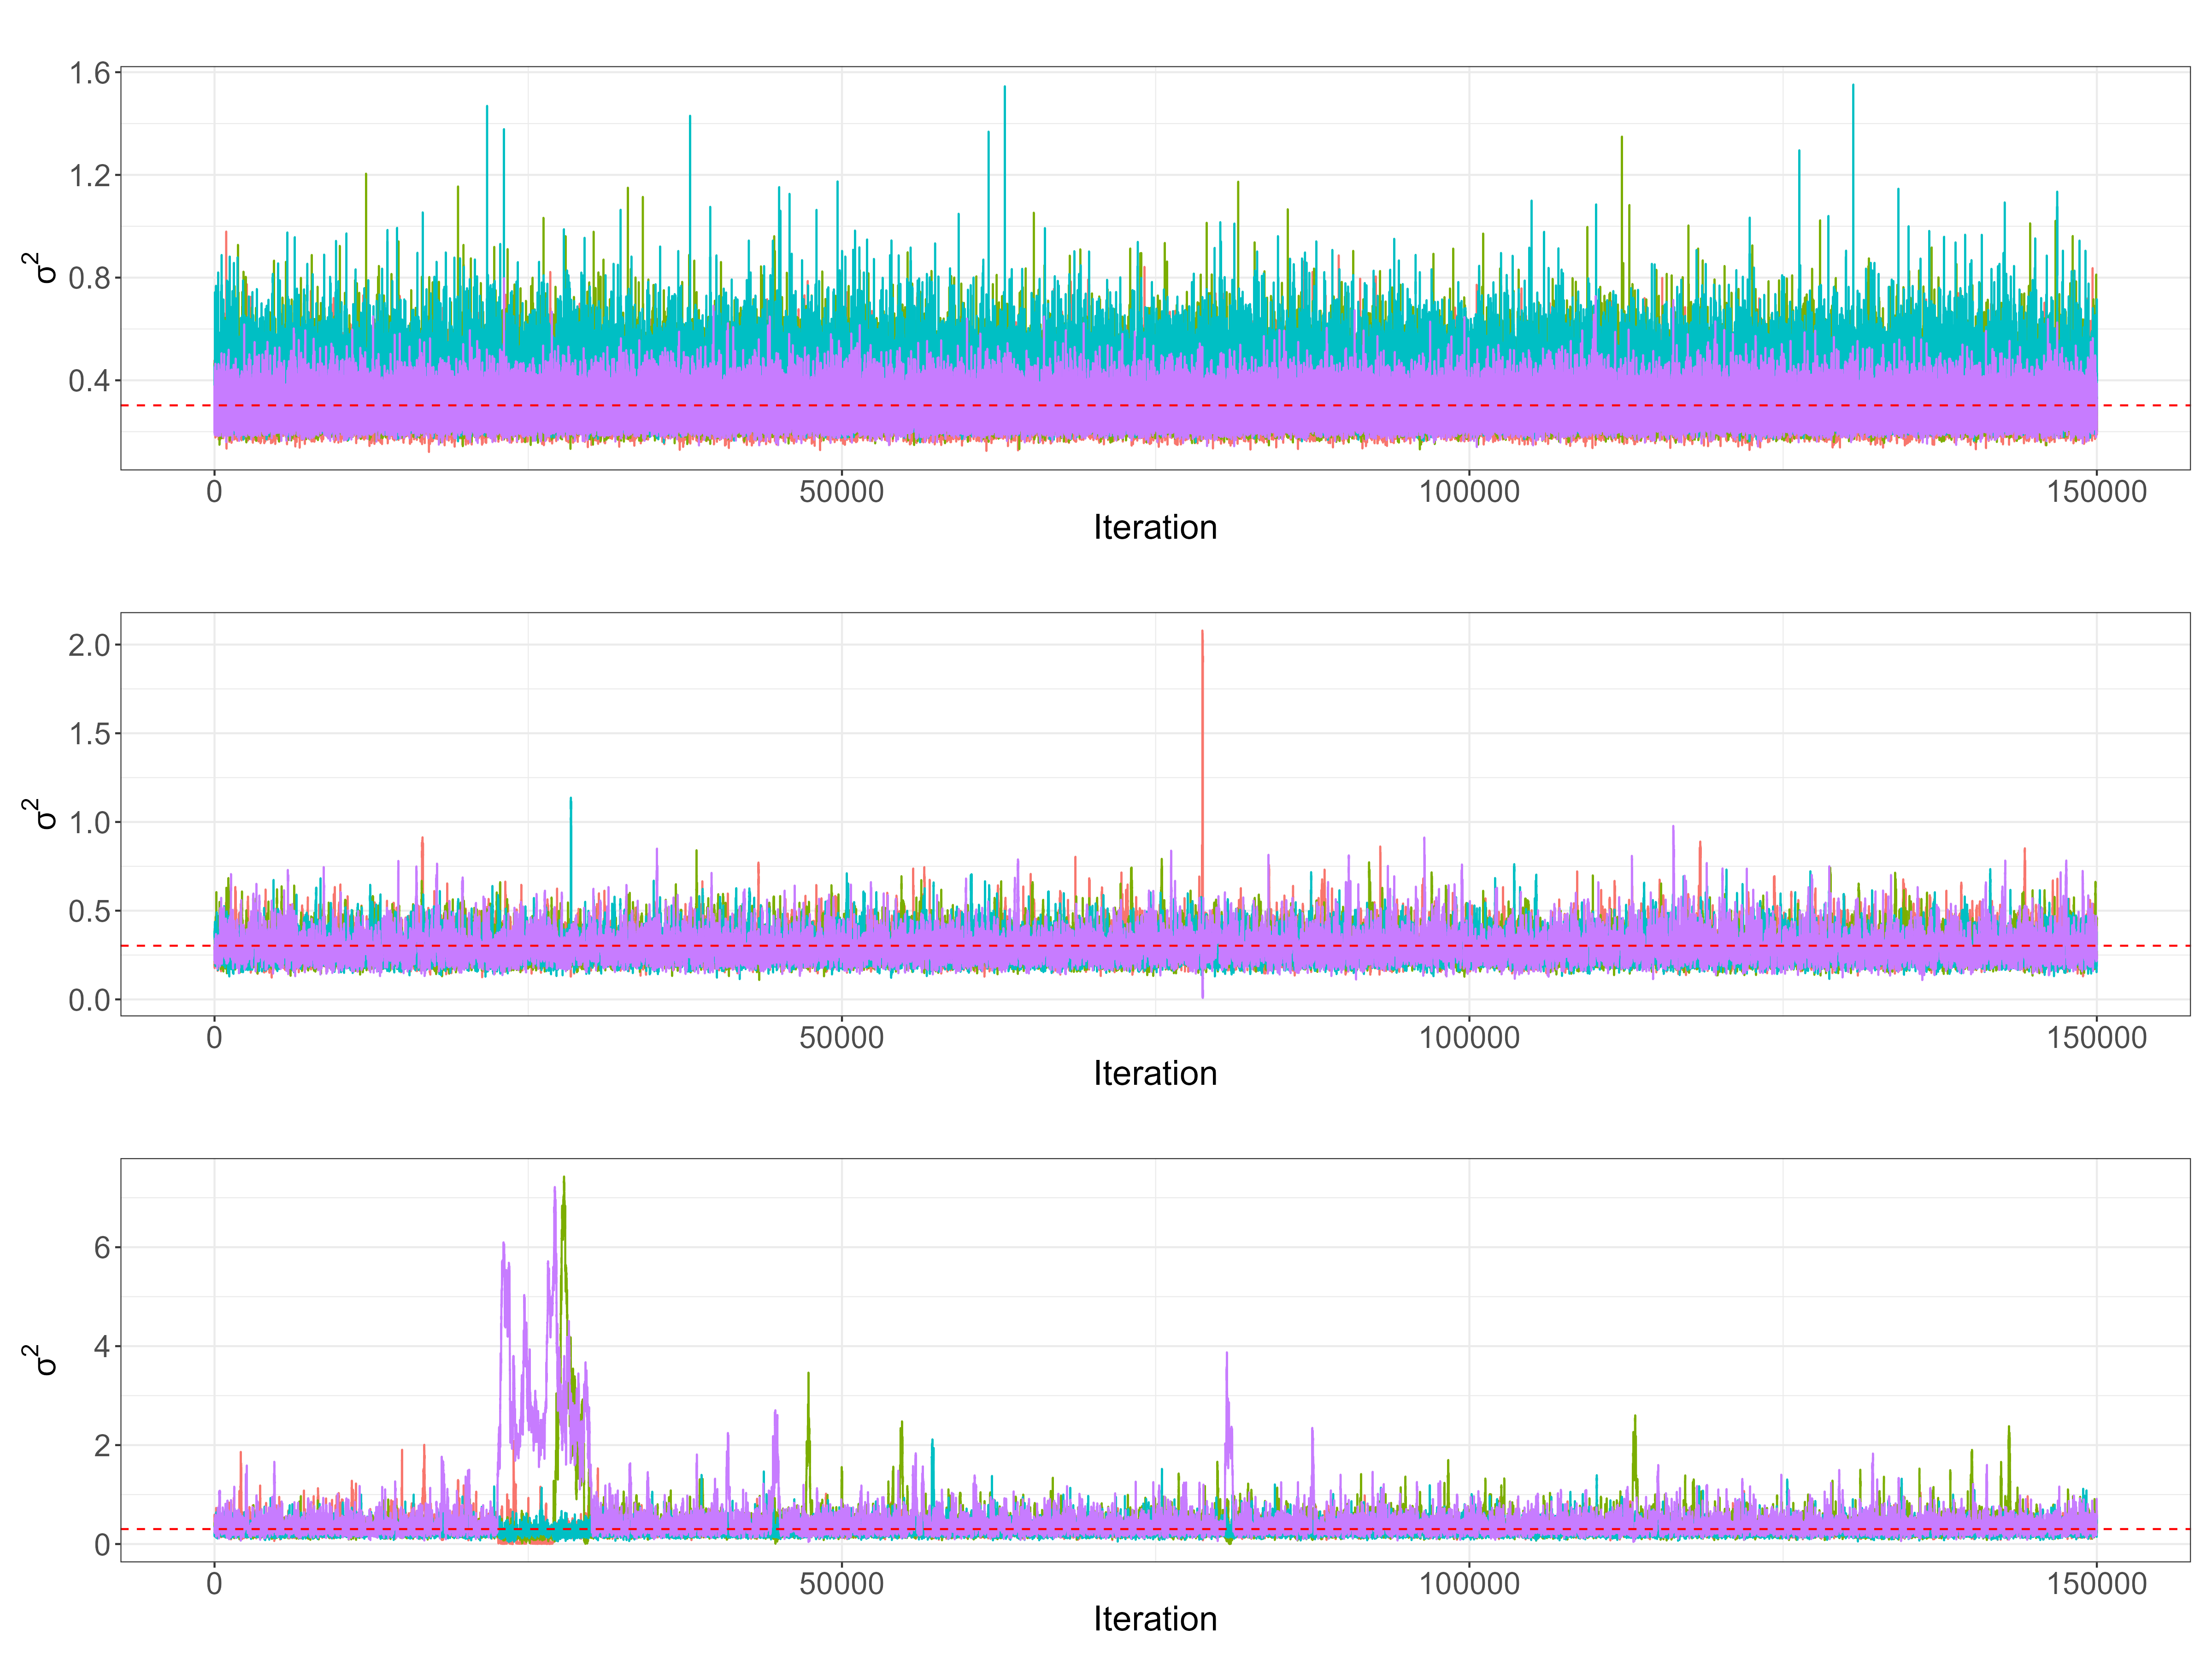
\includegraphics[scale=0.4]{figures/trace_sigma2_random_beta.png}
    \caption{\textbf{Trace plots for $\bsigma^2$.} The first row shows the trace for Gibbs sampling, the second 
    row for parallel tempering, and the third row for tempered transitions. Each color represents a different 
    component. The dashed lines indicate the true parameter values.}
    \label{fig:trace_plots_sigma}
\end{figure}

\begin{figure}[!ht]
    \centering
    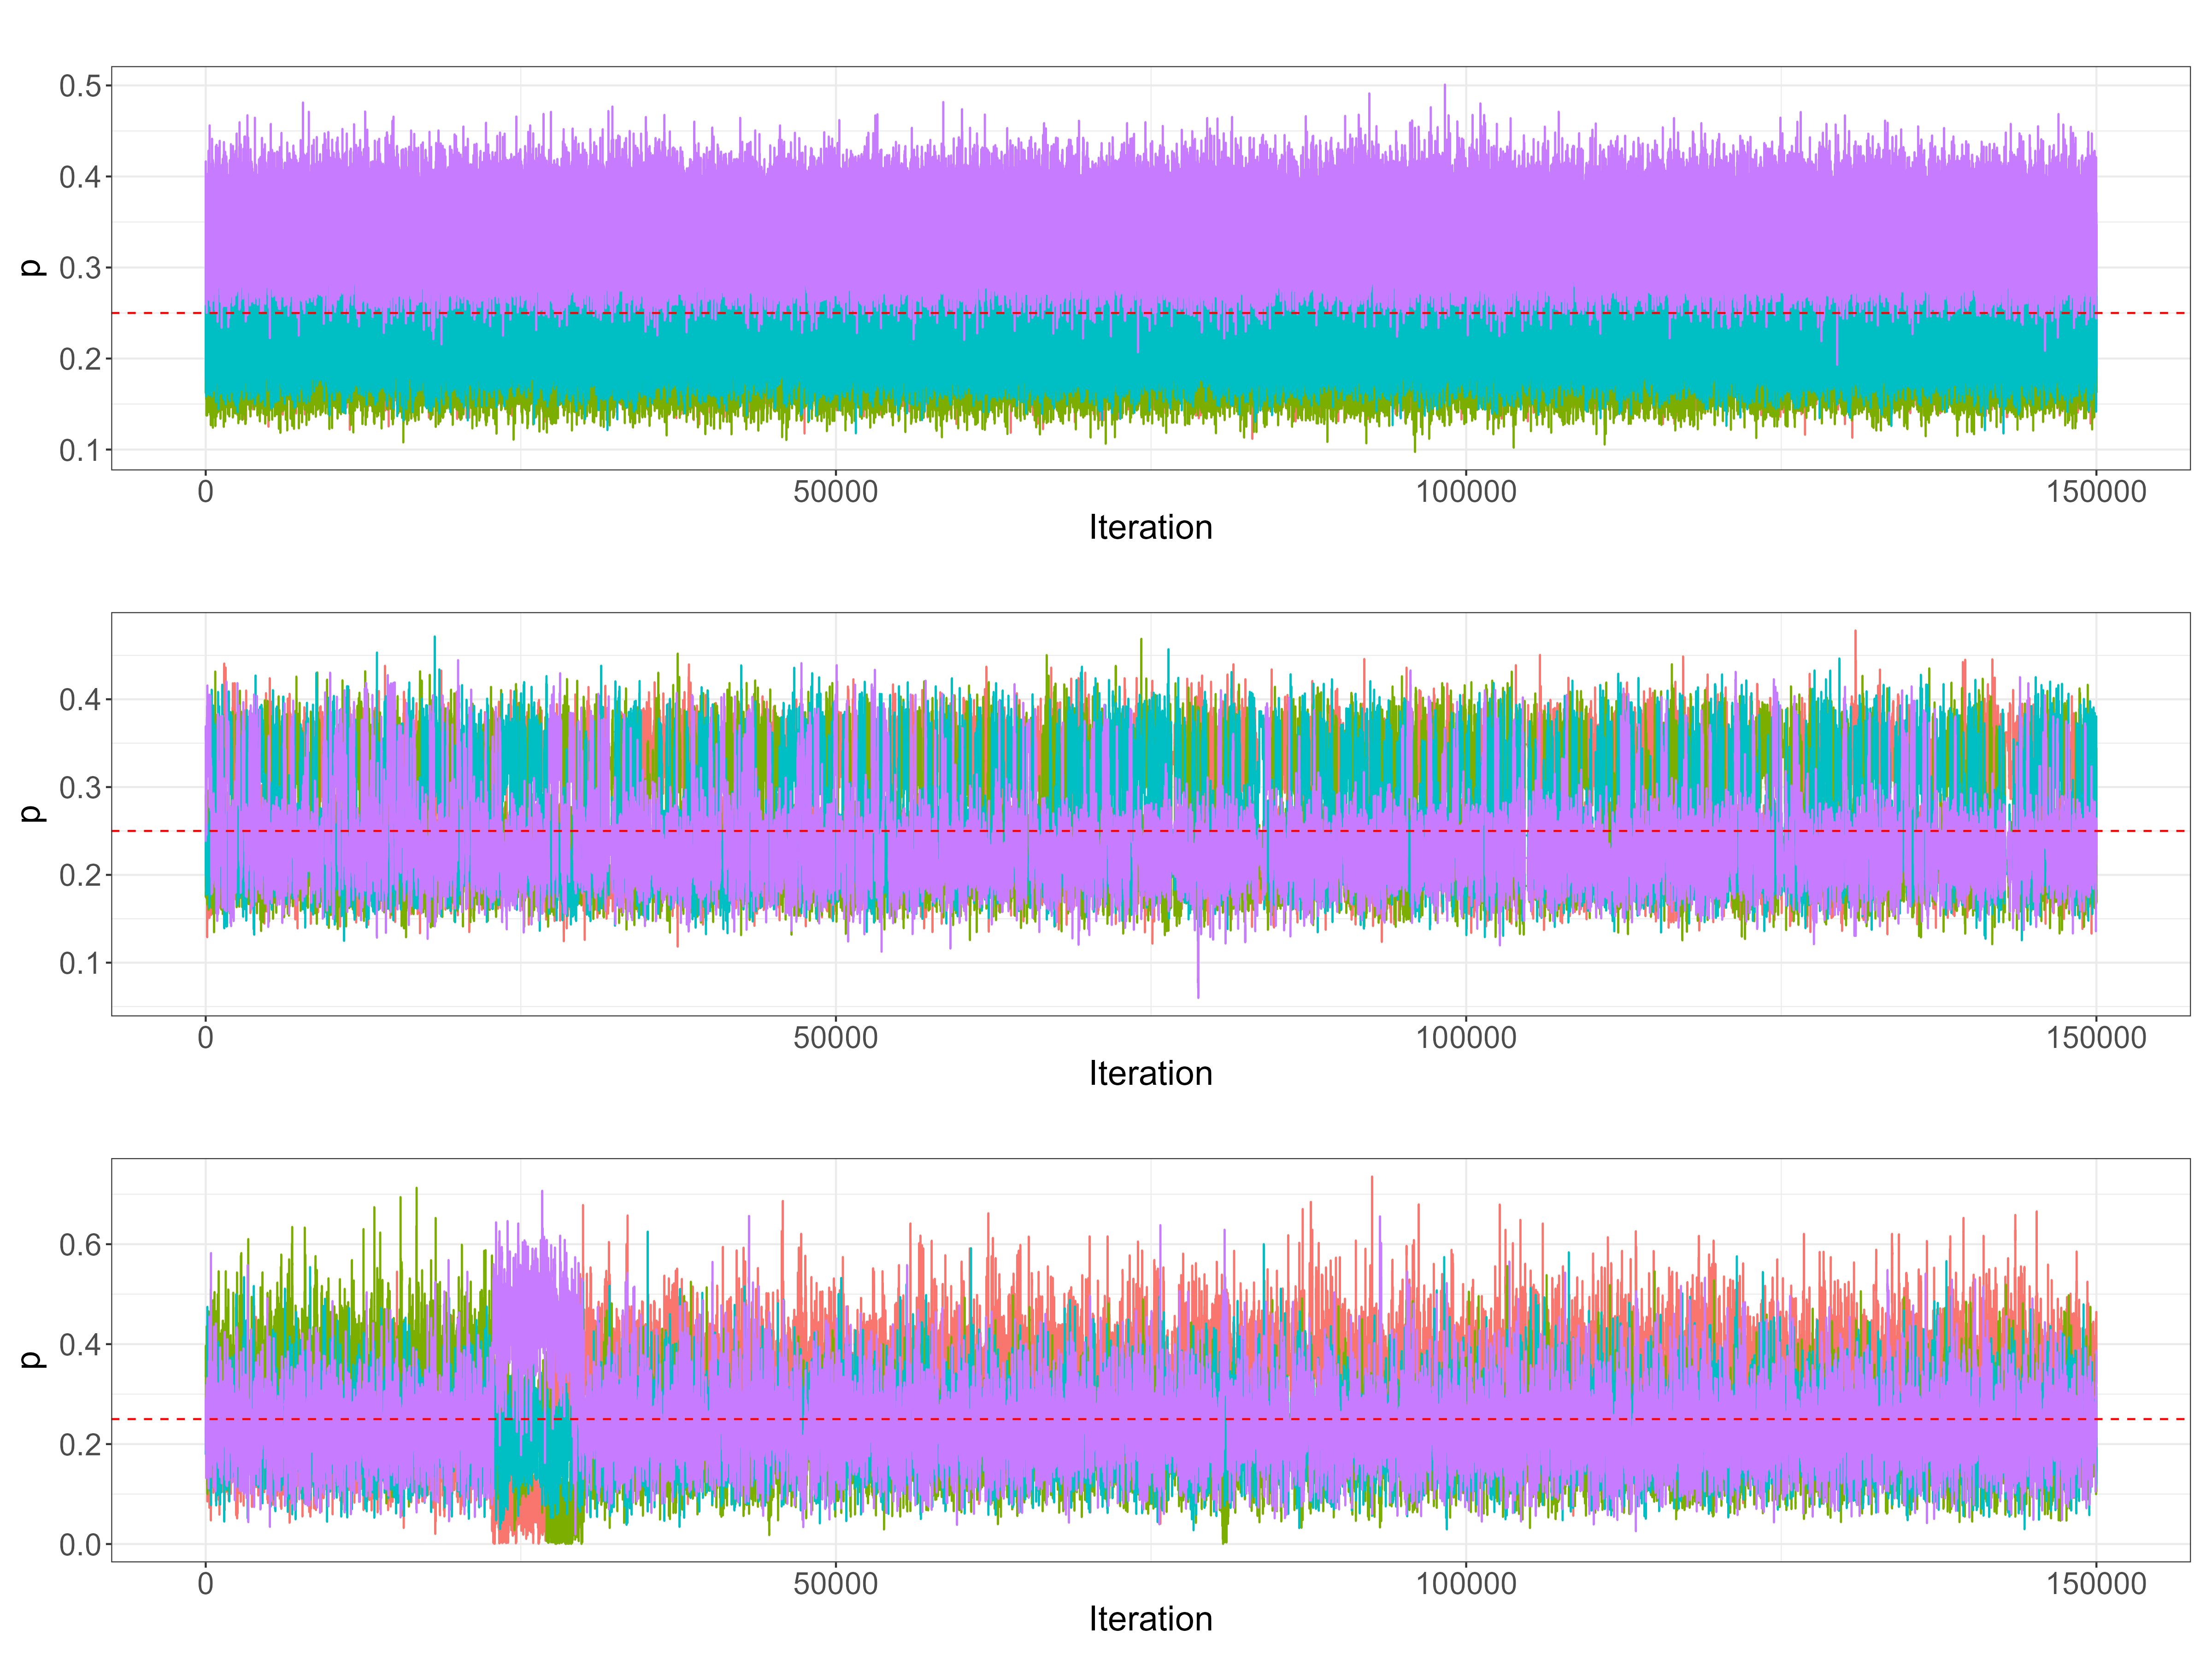
\includegraphics[scale=0.4]{figures/trace_p_random_beta.png}
    \caption{\textbf{Trace plots for $\bpi$.} The first row shows the trace for Gibbs sampling, the second row for
    parallel tempering, and the third row for tempered transitions. Each color represents a different component. 
    The dashed lines indicate the true parameter values.}
    \label{fig:trace_plots_pi}
\end{figure}

Next, we show the posterior distributions for the parameters $\bmu$, $\bsigma^2$, and $\bpi$ after applying
the identifiability constraints to the samples obtained from the three methods in the figures 
\ref{fig:posterior_mu}, \ref{fig:posterior_sigma}, and \ref{fig:posterior_pi}.

\begin{figure}[!ht]
    \centering
    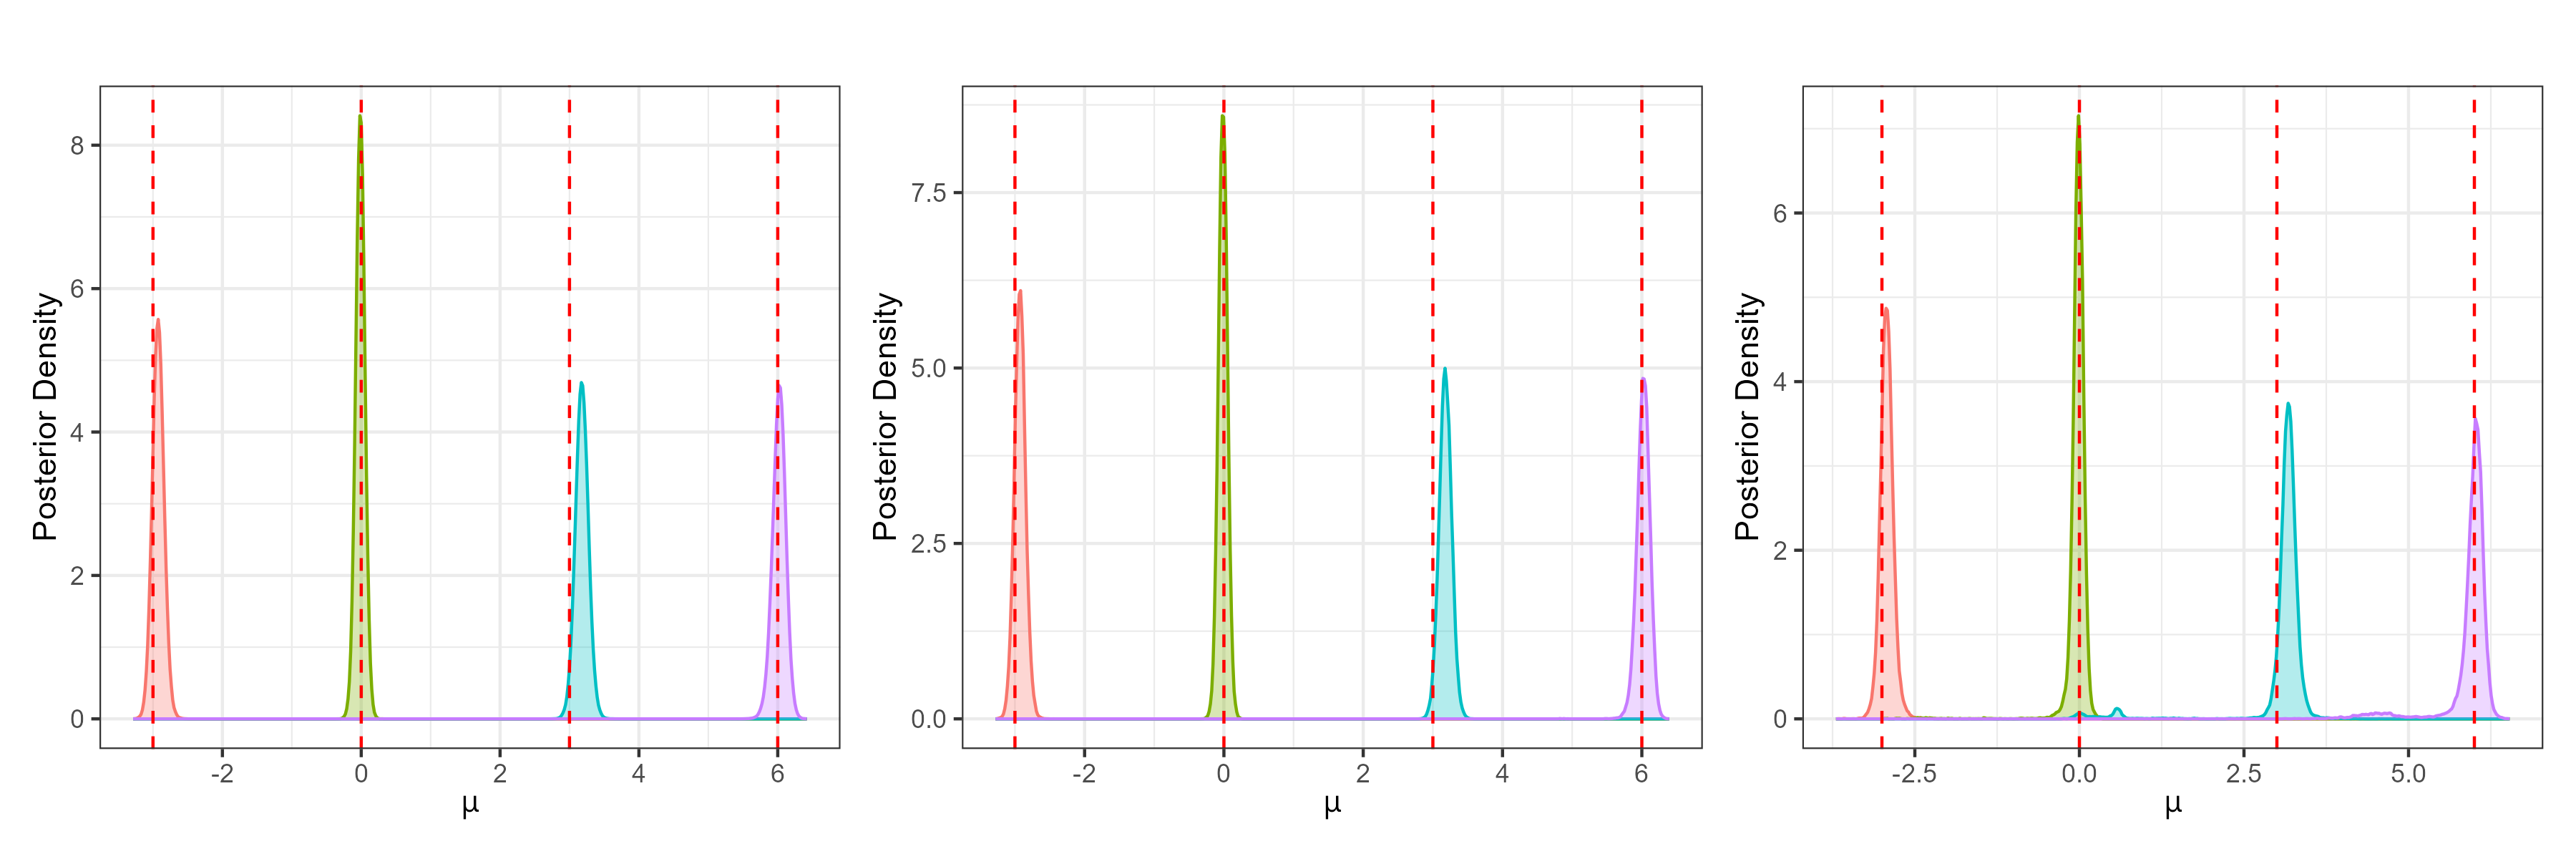
\includegraphics[scale=0.55]{figures/post_mu_random_beta.png}
    \caption{\textbf{Posterior distributions for $\bmu$.} The first column shows the posterior for Gibbs sampling,
    the second column for parallel tempering, and the third column for tempered transitions. Each color
    represents a different component. The dashed lines indicate the true parameter values.}
    \label{fig:posterior_mu}
\end{figure}

\begin{figure}[!ht]
    \centering
    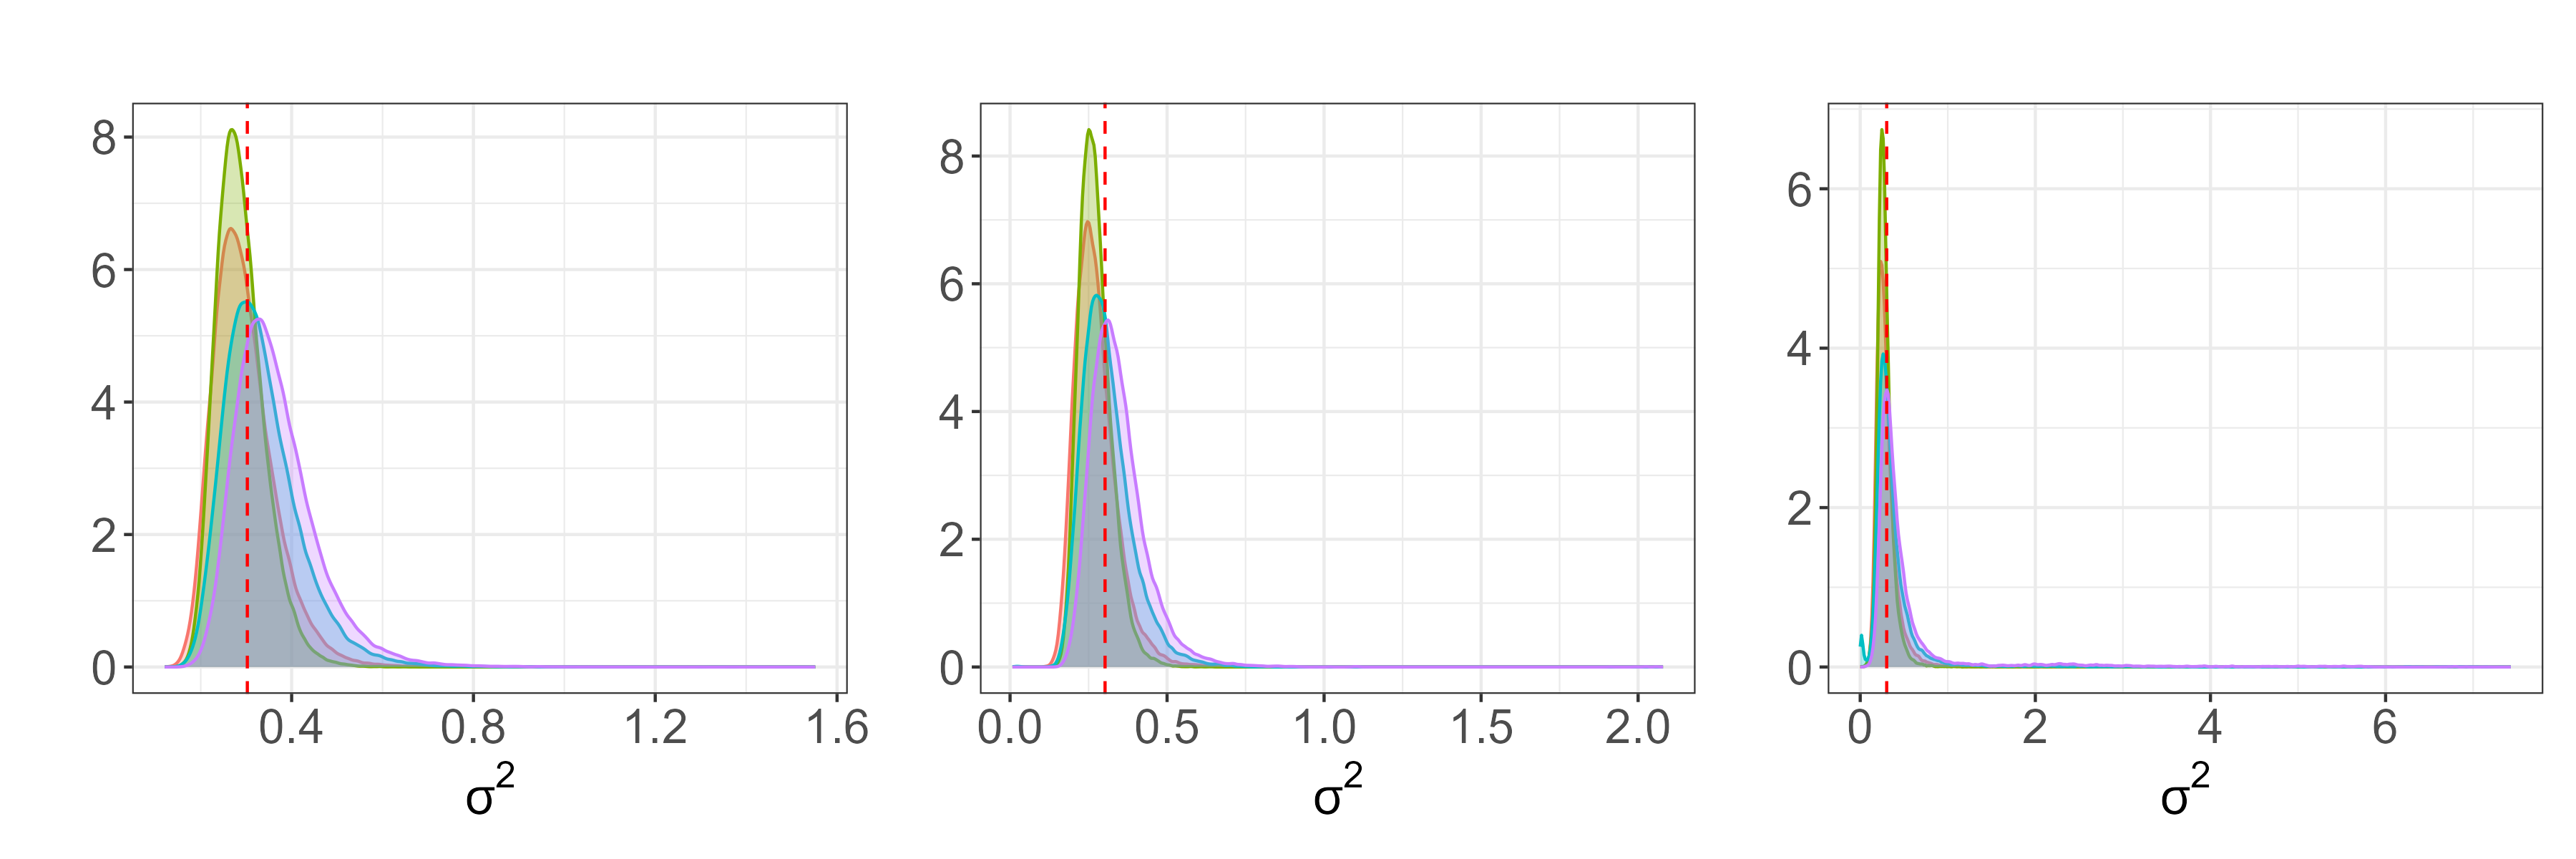
\includegraphics[scale=0.55]{figures/post_sigma2_random_beta.png}
    \caption{\textbf{Posterior distributions for $\bsigma^2$.} The first column shows the posterior for Gibbs 
    sampling, the second column for parallel tempering, and the third column for tempered transitions. Each color
    represents a different component. The dashed lines indicate the true parameter values.}
    \label{fig:posterior_sigma}
\end{figure}

\begin{figure}[!ht]
    \centering
    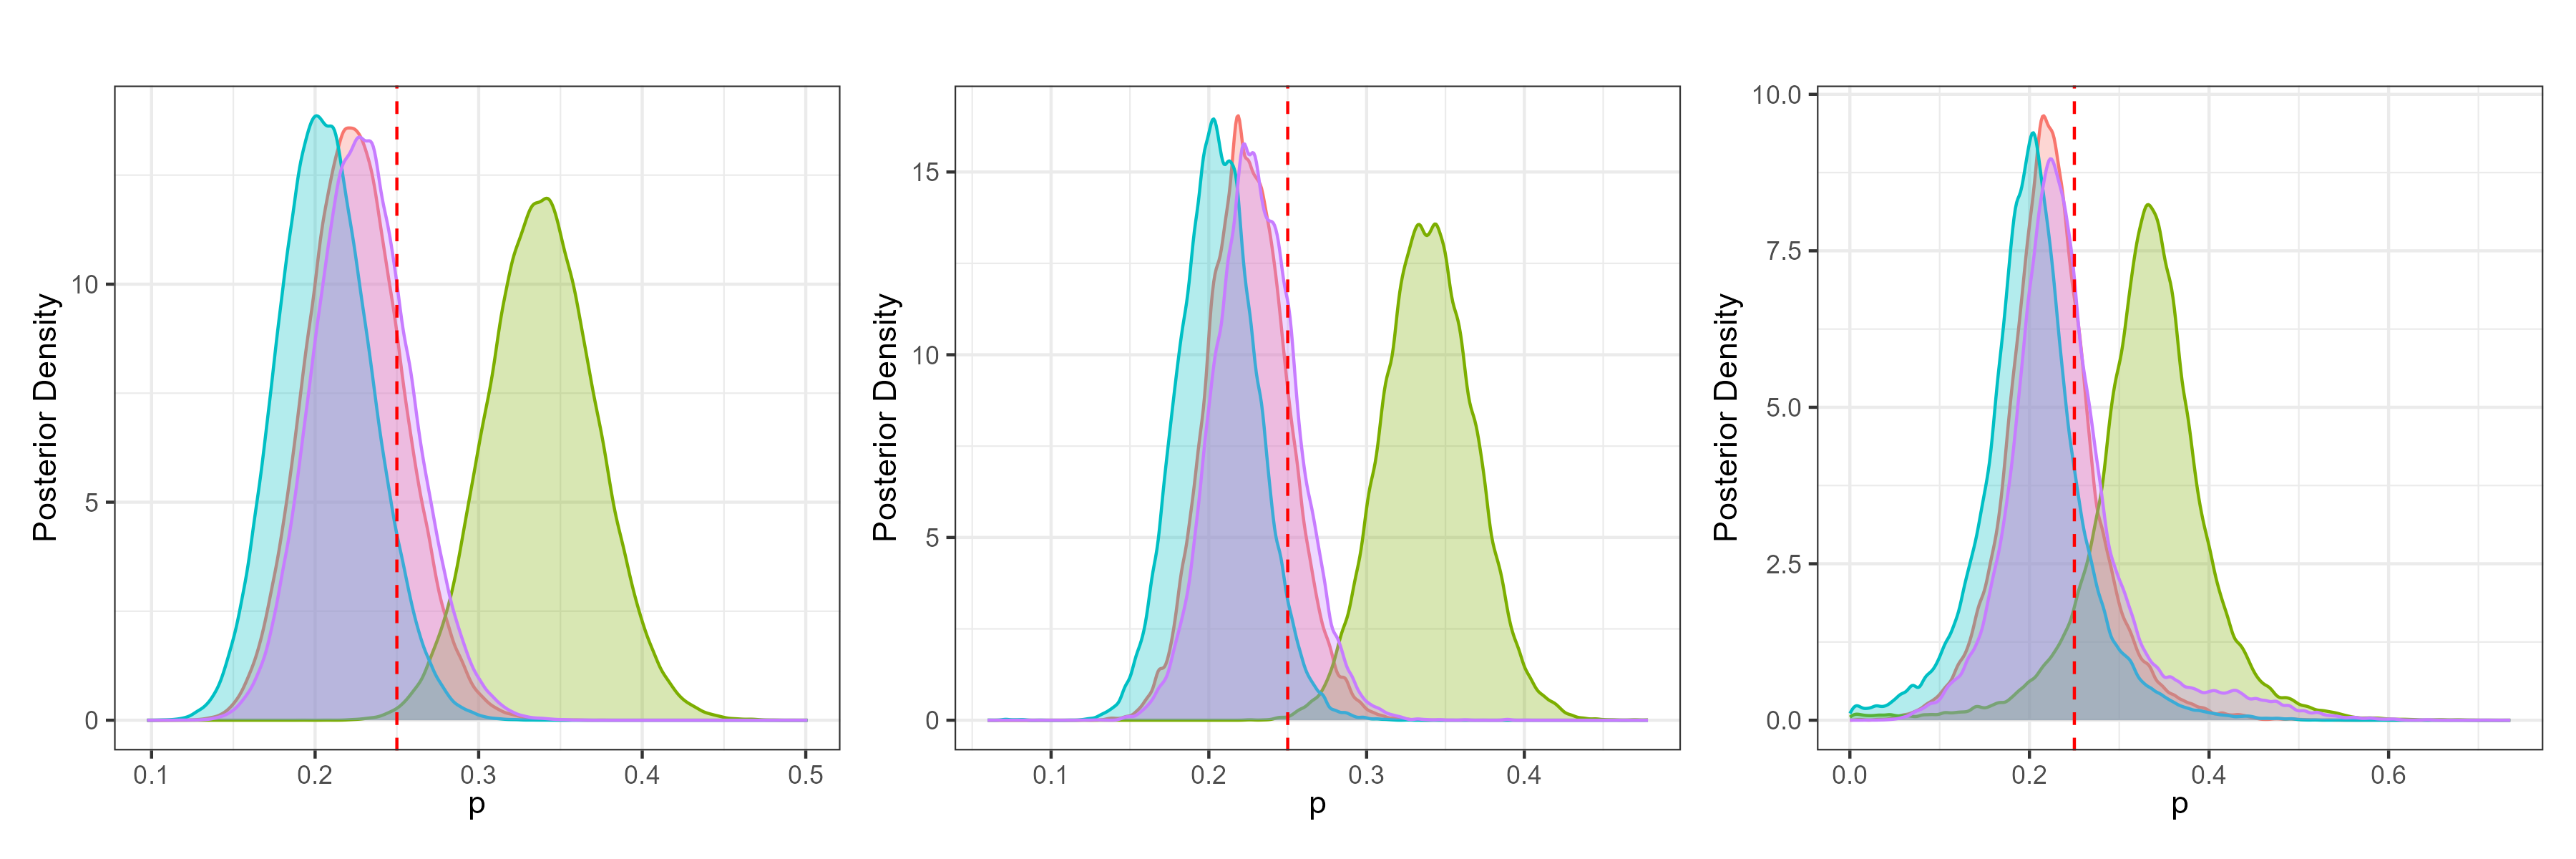
\includegraphics[scale=0.55]{figures/post_p_random_beta.png}
    \caption{\textbf{Posterior distributions for $\bpi$.} The first column shows the posterior for Gibbs sampling,
    the second column for parallel tempering, and the third column for tempered transitions. Each color
    represents a different component. The dashed lines indicate the true parameter values.}
    \label{fig:posterior_pi}
\end{figure}

Lastly, we show the acceptance rates for the three methods in the table \ref{tab:acceptance_rates} and 
the effective sample sizes in the table \ref{tab:effective_sample_sizes}.

\begin{table}[!ht]

\caption{\textbf{Acceptance rates by method.}}
\centering
\begin{tabular}[t]{lrrr}
\toprule
Method & $\mu$ & $\sigma^2$ & $\pi$\\
\midrule
Gibbs & 1.000 & 1.000 & 1.000\\
Parallel Tempering & 0.265 & 0.629 & 0.258\\
Temperated Transition & 0.215 & 0.377 & 0.362\\
\bottomrule
\end{tabular}
\label{tab:acceptance_rates}
\end{table}

\begin{table}[!ht]

\caption{\textbf{Effective sample sizes by method.}}
\centering
\begin{tabular}[t]{llll}
\toprule
Method & Gibbs & Parallel Tempering & Temperated Transition\\
$\mu_1$ & 129953 & 1005 & 9 \\
$\mu_2$ & 124791 & 1046 & 10\\
$\mu_3$ & 100228 & 968 & 5239\\
$\mu_4$ & 135154 & 1013 & 121\\
\addlinespace
$\sigma_1^2$ & 101667 & 2942 & 2289\\
$\sigma_2^2$ & 88399 & 3326 & 141\\
$\sigma_3^2$ & 72239 & 3630 & 3862\\
$\sigma_4^2$ & 106736 & 3168 & 80\\
\addlinespace
$\pi_1$ & 144709 & 1249 & 642 \\
$\pi_2$ & 138560 & 1346 & 721 \\
$\pi_3$ & 139232 & 1236 & 11194 \\
$\pi_4$ & 146301 & 1275 & 1070 \\
\bottomrule
\end{tabular}
\label{tab:effective_sample_sizes}
\end{table}

\section{Discussion and Conclusion}

In this paper, we explored the challenges of sampling from multimodal posteriors in Bayesian inference, 
focusing on the label switching problem. We discussed how standard MCMC methods, such as Gibbs sampling,
struggle with local modes and poor mixing in this context. We then introduced several advanced techniques,
including simulated tempering, parallel tempering, and tempered transitions, which improve exploration of the
posterior landscape. Also, we discussed how these methods can be combined with relabeling algorithms to address
the label switching problem. Then we presented a case study using simulated data from a random beta model, 
demonstrating the effectiveness of these methods in sampling from multimodal posteriors. 

We found that while Gibbs sampling does not move between modes, both parallel tempering and tempered transitions
are able to explore the multimodal posterior effectively, especially for the parallel tempering method. We also
observed that the tempered transitions method has a limited movement between modes, maybe due to the choice of
temperatures and the proposal distributions. The acceptance rates were significantly good for all methods, but
the effective sample sizes were much lower for the tempered transitions method, indicating that there is a
large autocorrelation in the samples and that the method does not explore the posterior well.

Despite the issues related, all methods were able to recover the true parameter values except for one of the 
components of $\bpi$. Furthermore, the identifiability constraints were effective in aligning the modes of the
posterior distributions in this case study. However, the larger computational cost of the tempered methods
and the need for a large number of iterations to achieve convergence are important considerations in practice. 
Also, we note that the choice of temperatures and proposal distributions is crucial for the performance of
tempered methods. In practice, it is often necessary to calibrate these parameters to ensure that the
sampler explores the posterior effectively. Future work could explore adaptive methods for selecting
temperatures and proposal distributions, as well as more sophisticated relabeling algorithms that can handle
more complex multimodal posteriors.

\clearpage

\bibliographystyle{plainnat}
\bibliography{references.bib}

\end{document}

